\section{Konzept}

Im Folgendem wird das Gesamtkonzept des Bankingserver beschrieben. Dies geschieht verteilt anhand von mehreren Sequenzdiagrammen.\\

\subsection{Grundkonzept}

Den Anfang macht hier das Diagramm zum Grundkonzept des Bankingservers.

\begin{figure}
\centering
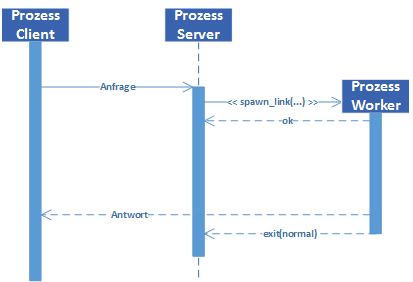
\includegraphics{/konzept/Allgemein}
\caption{Das Grundkonzept des kompletten Bankingservers}
\label{fig:grundkonzept}
\end{figure}

Der Startzustand besteht darin, dass Client so wie Server gestartet sind. Der Server ist kurz darauf in seinem Wartezustand, bei dem er auf eintreffende Nachrichten wartet.\\
Sobald der Client eine Anfrage an den Server richtet, wie z.B. "Konto erstellen", startet dieser einen Arbeitsprozess. Dieser neue Arbeitsprozess, oder auch Worker, erhält während seines Aufrufes alle notwendigen Daten, die er zur Erfüllung seiner Aufgabe benötigt. Dazu zählt auch die ProzessID des Clients.\\
Der Server erhält nach dem erfolgreichen Start des Workers ein ''ok'' zurück.\\
Der arbeitende Prozess ist nun damit beschäftigt die Aufgabe des Clients zu bearbeiten. So lange dies geschieht, bleibt der Server weiterhin erreichbar für neue Anfragen (dazu später mehr).\\
Sobald der Worker fertig mit seiner Arbeit ist, sendet er eine Antwort, welche eine Erfolgsmeldung und mögliche Kontodaten enthält, an den Client. Dieser kann die Nachrichten wie gewohnt über den \textbf{receive} - Befehl auslesen.\\
Der Server hingegen erhält bei der Beendigung des Workers ein normales ''exit'', welches signalisiert, dass der arbeitende Prozess sich ordnungsmäßig beendet und somit seine Aufgabe erfüllt hat.

\subsection{Multiclient Konzept}

Die Anfragen, welche an dem Server gestellt werden, sollen möglichst schnell abgearbeitet werden. Dazu ist es erforderlich das Abarbeiten dieser Anfragen zu parallelisieren.

\begin{figure}
\centering
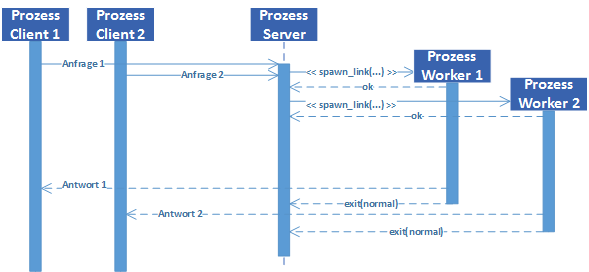
\includegraphics{/konzept/Multiclient}
\caption{Bankingserver mit mehreren parallelen Clients}
\label{fig:multiclient}
\end{figure}

In diesem Sequenzdiagramm befinden sich zwei Clients, welche fast zeitgleich, jeweils eine Anfrage an den Server richten.\\
Der Server bekommt zu erst die ''Anfrage 1'' von ''Client 1'', welche somit auch als erstes abzuarbeiten ist. Dazu wird, wie schon im Grundkonzept beschrieben, ein Worker (hier ''Worker 1'') gestartet.\\
So lange der Server mit dem \textit{spawn\_link} für ''Worker 1'' benötigt, wird ''Anfrage 2'' nicht bearbeitet. Diese Verzögerung ist jedoch minimal, muss allerdings trotzdem in kauf genommen werden.\\
Darauf folgend wird ''Anfrage 2'' so schnell wie möglich bearbeitet. Dies geschieht hier in ''Worker 2''.\\
Die Clients erhalten, nach der Abarbeitung ihrer entsprechenden Anfragen, nach schon bekanntem Verfahren, die jeweiligen Antworten von den Workern.

\subsection{Störungs Konzept}

Eine der Aufgaben des Projekts war eine Störquelle einzubauen, welche den normalen Betrieb der Worker beeinträchtigen soll. Dieses wird dadurch realisiert, dass ein Störprozess vereinzelt Worker beendet, bevor sie mit ihren Aufgaben fertig sind.\\

\subsubsection{Das Wirken der Störung}

Das folgende Diagramm zeigt wie besagter Prozess den ersten laufenden Worker beendet, denn zweiten allerdings ohne einzugreifen arbeiten lässt.\\

\begin{figure}
\centering
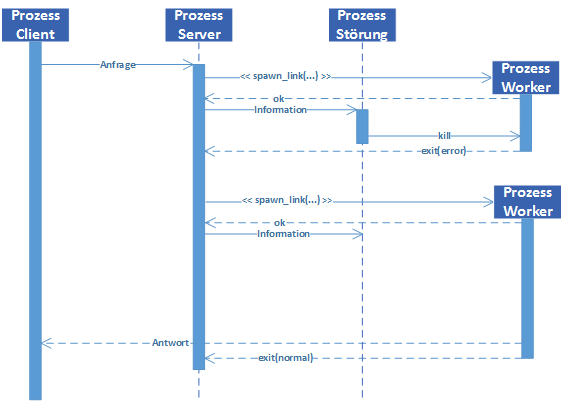
\includegraphics{/konzept/Stoerung}
\caption{Bankingserver mit eingebauter, aktiver Stoerungsquelle}
\label{fig:stoerung}
\end{figure}

Client und Server verfahren vorerst, nach bekanntem Vorgehen. Nachdem allerdings der neue Worker sein ''ok'' an den Server zurückschickt, informiert der Server, die Störquelle über den neuen Arbeitsprozess. \\
Dieses Verhalten des Servers ist normalerweise nicht in endgültiger Software enthalten, und ist hier nur erforderlich um Störungen und Fehlverhalten zu simulieren.\\
Der Störprozess entscheidet nun, dass dieser Worker von ihm beendet wird (''kill''). In Folge dessen erhält der Server, wegen der Verlinkung mit dem Worker, ein ''exit(error)''. Dies signalisiert dem Bankingserver, dass der Arbeitsprozess sich mit einem Fehler beendete. Wenn der Worker seine Aufgabe noch nicht erledigen konnte, bevor er vom Störprozess beendet wurde, ist die Anfrage des Clients immer noch ausstehend. In diesem Beispiel wird von diesem Fall ausgegangen.\\
Es ist also erforderlich, dass der gleiche Arbeitsprozess, mit den gleichen Parameter, erneut gestartet wird.

\subsubsection{Das Ausgleichen der Störung}

Nachdem die Unterbrechung durch den Störungsprozess verursacht wurde, muss dies erkannt und aufgelöst werden.\\
Wie anhand von dem Diagramm~\ref{fig:stoerung} erklärt wurde, gibt ein von dem Störungsprozess beendeter Worker ein \textit{exit(error)} an den Server zurück. Dieser erkennt diese Meldung und hat nun die Aufgabe potenziellen Schaden zu erkennen.\\
Um die Suche nach nicht ausgeführten Anfragen durchzuführen werden die zugehörigen Transaktionslisten durchsucht.

\paragraph{Transaktionsliste des Servers}

Die Transaktionsliste des Servers enthält sämtliche Transaktionen, welche derzeit durchgeführt werden. Wurde eine Anfrage erfolgreich bearbeitet wird der dazugehörige Eintrag dieser Liste gelöscht.\\
Der Aufbau eines Tupels der Liste ist folgende:

\begin{lstlisting}
%
%{ TransaktionsID,  { Aktion, [ ClientPID | Arguments ] ] } }
%
\end{lstlisting}

\begin{itemize}
	\item ''TransaktionsID'': Ist eine eindeutige ID, welche eine Transaktion markiert.
\end{itemize}
Das darauf folgende Tupel ist dafür die restlichen Informationen zu speichern, welche unter Umständen dafür benötigt werden um Worker erneut zu starten.
\begin{itemize}
	\item ''Aktion'': Speichert die Aufgabe, welche durchgeführt werden soll.
	\item ''ClientPID'': Steht für die Prozess ID des Clients, welcher die Anfrage gestellt hat.
	\item ''Arguments'': Der Rest der Liste besteht aus den Argumenten für den Worker, welche die Aufgabe ausführen muss.
\end{itemize}

\paragraph{Transaktionen in der allgemeine Kontenspeicherung}

Im \textit{dets} - Modul für die allgemeine Kontenspeicherung wird jede durchgeführte Transaktion bei den einzelnen Konten gespeichert. Die angehängten Transaktionslisten sind folgendermaßen aufgebaut:

\begin{lstlisting}
% 
% {TransaktionsID,
%	Aktion,
%	{zeit, Datum, Uhrzeit},
%	{notizen, Notizen},
%	{wer, Kontonummer},
%	{wert, Betrag}
% }
%  
\end{lstlisting}

\begin{itemize}
	\item ''TransaktionsID'': Diese ID eindeutig markiert einzelne Transaktionen und stimmt mit der TransaktionsID der Transaktionsliste des Servers überein.
	\item ''Aktion'': Speichert die durchgeführte Aktion.
	\item Tupel ''Zeit'': Speichert den Zeitpunkt in dem die Aktion ausgeführt wurde.
	\item Tupel ''Notizen'': Speichert zusätzliche Notizen bei einzelnen Transaktionen.
	\item Tupel ''Wer'': Speichert die Information von welchem Konto die Transaktion ausgelöst wurde. Dies ist vor allem bei Überweisungen wichtig.
	\item Tupel ''Betrag'': Speichert den Betrag, welcher bei der Transaktion bewegt wurde.
\end{itemize}
Sobald der Server die Nachricht eines sich fehlerhaft beendeten Workers erhält, überprüft er, ob die Transaktion welcher der Worker auszuführen hatte, erledigt wurde. Dies geschieht dadurch, dass der Server die Transaktions - ID des Workers in der Transaktionsliste des betreffenden Kontos sucht. Kann er diese finden, wurde die Anfrage vor dem Wirken der Störung durchgeführt. Dies bedeutet, dass die Aufgabe des Workers nicht wiederholt werden muss. Wird die entsprechende Transaktions - ID nicht gefunden, wurde die Anfrage noch nicht bearbeitet. Ein gleicher Worker muss gestartet und die Aufgabe wiederholt werden.

%\subsection{Client}
Das Client Modul ist die eigentliche Schnittstelle der Applikation für den Benutzer. Mittels des Moduls kann ein Nutzer möglichst komfortabel Anfragen an den Banking Server schicken, ohne sich dabei Gedanken machen zu müssen, wie der Server an sich aufgebaut ist und angesprochen werden müsste.\\
Um einen Client zu starten, wird die Funktion \textit{start} aufgerufen, welche als einzigen Parameter den Namen, auf den der Client registriert werden soll entgegennimmt. Alle weiteren Aktionen erfolgen ausschließlich über Nachrichten, die an den registrierten Client geschickt werden. Dies hat den Vorteil, das innerhalb einer Shell mehrere Clients gleichzeitig benutzt werden können.\\
Die Funktion des Clients soll folgender Aufruf aus der Shell verdeutlichen:
\begin{lstlisting} 
 (bc@localhost)1> bc:start(client1).
 Banking Client wurde gestartet
 ok
 (bc@localhost)2> client1 ! konto_anlegen.
 konto_anlegen
 OK: 6
\end{lstlisting}
Im ersten Schritt, wird ein neuer Client mit dem Namen ''\textit{client1}'' erzeugt. Danach ist es möglich, über den Client Aufträge an den Server zu schicken.\\ 
So wird in Schritt drei mittels des Befehls ''\textit{konto\_anlegen}'' ein neues Konto angelegt. Als Antwort für die Anfrage bekommt der Client ''\textit{OK: 6}'' zurück. Dies bedeutet, das die Anfrage korrekt ausgeführt wurde, und ein neues Konto mit der Kontonummer \textit{6} angelegt wurde.\\
Die verschiedenen Befehle, die der Client ausführen kann und deren Syntax sind in der nachfolgenden Tabelle aufgelistet.\\
\begin{table}[H]
\caption{Client Funktionen}
\begin{center}
\begin{tabular}[t]{l|l}
\textbf{Funktion} 	& \textbf{Syntax} \\
Konto anlegen 			& client ! \textit{konto\_anlegen}\\
Konto löschen 			& client ! \{\textit{konto\_loeschen}, Kontonummer\}\\
Kontostand abfragen 	& client ! \{\textit{kontostand\_abfragen}, Kontonummer\}\\
Historie ausgeben 		& client ! \{\textit{historie}, Kontonummer\}\\
Geld einzahlen			& client ! \{\textit{geld\_einzahlen}, Kontonummer, Betrag, Verwendungszweck\}\\
Geld auszahlen 			& client ! \{\textit{geld\_auszahlen}, Kontonummer, Betrag\}\\
Geld überweisen 		& client ! \{\textit{geld\_ueberweisen}, ZielKontonummer, UrsprungsKontonummer, Betrag\}\\
Dispokredit beantragen 	& client ! \{\textit{dispokredit\_beantragen}, Kontonummer\}\\
Konto sperren 			& client ! \{\textit{konto\_sperren}, Kontonummer\}\\
Konto entsperren 		& client ! \{\textit{konto\_entsperren}, Kontonummer\}\\
Client beenden 			& client ! \textit{stop}
\end{tabular}
\end{center}
\end{table}
Es ist zu beachten, dass die Nachrichten stets an den registrierten Client-Namen geschickt werden müssen. Der in der Tabelle verwendete Client-Name (\textit{client}) dient lediglich der Veranschaulichung.\\
Funktionen, die Übergabeparameter enthalten, müssen grundsätzlich als Tupel geschickt werden und zwingend alle Argumente enthalten. Wird dem Client eine Nachricht geschickt, deren Kommando er nicht kennt, oder deren Argumente unvollständig sind, quittiert er diese mit \textit{''Unbekanntes Kommando''}.\\
Die Rückgabe des Clients ist entweder positiv oder negativ. Konnte die Anfrage erfolgreich bearbeitet werden, gibt der Client ''\textit{OK: }'' mit den abgehangenen Rückgabewerten des Worker-Prozesses zurück. Im negativ Fall gibt der Client ''\textit{Fehler: }'' mit den angehangenen Fehlerinformation des Workers-Prozesses zurück.\\
Als nicht erfolgreich werden lediglich fehlerhafte Anfragen gewertet, beispielsweise die Anfrage des Kontoguthabens zu einem nicht existierendem Konto. Fehlerhaftes Verhalten eines Worker-Prozesses, welches dazu führt, das für eine Anfrage ein Worker neu gestartet werden muss, bleibt für den Client verborgen.\\
Die eigentliche Anfrage an den Server erfolgt durch einen asynchronen Aufruf des Servers, wie folgender Codeausschnitt des Client Moduls zeigt.
\begin{lstlisting} 
loop() ->
 receive
      konto_anlegen ->
         gen_server:cast({bs, 'bs@localhost'}, {konto_anlegen, self()}),
         loop();
      {kontostand_abfragen, KontoNr} ->
         gen_server:cast({bs, 'bs@localhost'}, {kontostand_abfragen, self(), KontoNr}),
         loop();
		...
end.
\end{lstlisting}
Da es sich bei dem Server um einen generischen Server handelt, erfolgt der Aufruf mittels ''\textit{gen\_server(Name, Nachricht)}''. Der Server läuft auf einem anderem Node als der Client. Deshalb ist es notwendig, als Namen nicht nur den registrierten Namen des Servers anzugeben, sondern auch den Namen des Nodes ('bs@localhost'), auf dem dieser ausgeführt wird. Als Nachricht werden neben der Aktion die durchgeführt werden soll und die dazu nötigen Argumente auch die eigene Prozess Id übergeben, damit der Worker Prozess später an den Client eine Antwort schicken kann.
%\subsection{Server}
Das Server Modul dient der Interaktion von Client und Worker-Prozessen. Das Modul nutzt die ''gen\_server'' Funktionalität, welche eine möglichst einfache Client/Server Kommunikation ermöglicht.\\
Der Server wird mittels \\''\textit{bs:start(})'' gestartet. Diese Funktion ruft intern ''gen\_server:start\_link(ServerName, CallBackModule, Arguments, Options)'' auf, wie in folgendem Modulausschnitt zu sehen ist.
\begin{lstlisting}
 start() -> gen_server:start_link({local, ?MODULE}, ?MODULE, [], []).
\end{lstlisting}
Der Aufruf lässt erkennen, dass keine erweiterten Funktionalitäten des generischen Servers benutzt werden. Es wird lediglich der Name des Servers festgelegt, welcher gleich dem Modulnamen ist und der Name des Callback Moduls, welches dem eigenen Modul entspricht. Da für die Funktionalität des Banking Servers keine Initialisierungsdaten und Optionen benötigt werden, werden hierfür nur leere Listen übergeben.\\
Durch den Aufruf von ''\textit{gen\_server:start\_link}'', wird die Init Funktion des Banking Servers ausgeführt.
Innerhalb der Init Funktion wird das Flag ''\textit{trap\_exit}'' auf \textit{true} gesetzt. Dies führt dazu, dass vom Server aufgespannte Prozesse an ihn eine Nachricht senden, wenn sie beendet werden und er im Falle eines abgestürzten Prozesses nicht selber beendet wird. Zudem wird in der Init Funktion die Dets Datenbank geöffnet, welche die offenen Transaktionen verwaltet. Geschlossen wird die Datenbank erst wieder, wenn der Server innerhalb der ''\textit{terminate}'' Methode beendet wird.\\
Die Hauptaktivität des Banking Servers liegt in den Methodenaufrufen von ''\textit{handle\_cast(Name, Message)}''. Dies sind die Callback Funktionen der vom Client aufgerufenen ''\textit{gen\_server:cast(...)}'' Methoden. Für jeden Transaktionstyp existiert dabei eine ''\textit{handle\_call}'' Callback Methode. Wie diese im Detail aufgebaut sind, soll folgender Ausschnitt verdeutlichen.
\begin{lstlisting}
 handle_cast({geld_einzahlen, ClientPId, Kontonr, Verwendungszweck, Betrag}, LoopData) ->
   erzeuge_transaktion(geld_einzahlen, [ClientPId, Kontonr, Verwendungszweck, Betrag]),
   {noreply, LoopData};
\end{lstlisting}
Zu Erkennen ist, dass die Nachricht jeweils auf die auszuführende Transaktion gematched wird. Im dargestellten Fall auf ''\textit{geld\_einzahlen}''. Die Reihenfolge der Argumente ist im Wesentlichen stets die selbe. Nach der auszuführenden Aktion folgt die Client PID, mittels derer der Worker-Prozess später eine Antwort an den Client zurückschicken kann. Danach folgt falls, nötig die Kontonummer und anschließend weitere Argumente, die für die Ausführung der Aktion notwendig sind.\\
Innerhalb der Funktion wird die Methode ''\textit{erzeuge\_transaktion(Aktion, Args}'' aufgerufen, welche im folgenden Ausschnitt gezeigt wird.
\begin{lstlisting}
 erzeuge_transaktion(Action, Arg) ->
   TId = spawn_link(bw, init, []),
   dets:insert(transaction, {TId, {Action, Arg}}),
   TId ! [Action|Arg].
\end{lstlisting}
Die Funktion spannt den Worker Prozess auf und ruft die in ihm enthaltene Init Funktion auf. Die zurückerhaltene Prozess Id wird zusammen mit dem Transaktionstyp und den zusätzlichen Argumenten in der Transaktionsdatenbank gespeichert. Anschließend wird an den gestarteten Worker eine Nachricht mit der auszuführenden Transaktion und den Argumenten gesendet.\\
Wie bereits erwähnt, überwacht der Server die Worker-Prozesse, und bekommt eine Nachricht, falls sich ein solcher beendet. Hierbei wird zwischen einem normalen und einem fehlerhaften Beenden unterschieden. Wie dies getan wird zeigt folgender Ausschnitt aus dem Server-Modul.
\begin{lstlisting}
handle_info({'EXIT', TId, error}, LoopData) -> 
   io:format("Worker Exit: ~p (~p)~n", [error, TId]),
  ...
   {noreply, LoopData};

handle_info({'EXIT', PId, normal}, LoopData) -> 
   io:format("Worker Exit (not handled): ~p (~p)~n", [normal, PId]),
   dets:open_file(transaction, [{file, "db_transaction"}, {type, set}]),
   dets:delete(transaction, PId),
   dets:close(transaction),
{noreply, LoopData}.
\end{lstlisting}
Es ist ersichtlich, dass die Nachrichten, welche über die Beendigung eines Prozesses informieren mit der Callback Funktion ''\textit{handle\_info(Nachricht, LoopData)}'' abgehandelt werden. Übergeben wird dabei in jedem Fall das Atom \textit{'Exit'}, die Prozess Id des beendeten Prozesses und die Art der Beendigung als Atom.\\
Ist die Beendigungsart als ''\textit{normal}'' angegeben, bedeutet dies, dass der Prozess ordnungsgemäß durchgelaufen ist. Sollte dies der Fall sein, wird aus der Transaktionsdatenbank des Servers die Transaktion, für welche der beendete Prozess zuständig war, entfernt. So stehen innerhalb der Datenbank nur Transaktionen, die noch ausgeführt werden müssen, oder gerade ausgeführt werden.\\
Ist ein Prozess ''gekillt'' worden, oder abgestürzt, lautet der Beendigungsgrund ''\textit{error}''. Da nicht klar ist, ob der Prozess zum Zeitpunkt seines Absturzes bereits die Transaktion ausgeführt hat oder nicht, muss zunächst in der Datenbank der Worker geprüft werden, ob die Transaktion auf dem entsprechenden Konto bereits gespeichert wurde. Ist dies der Fall, kann die Transaktion aus der Transaktionsliste des Servers gelöscht werden. Ansonsten muss diese neu gestartet werden.\\
Besondere Aufmerksamkeit muss man Transaktionen widmen, die zwei Konten gleichzeitig bearbeiten. Darunter fällt eine Überweisung. Hier wird von einem Konto zunächst Geld abgebucht und daraufhin auf das andere Konto eingezahlt. Ist der Worker-Prozess genau zwischen diesen zwei Schritten abgestürzt, kann die Überweisungstransaktion nicht einfach erneut ausgeführt werden, da dies dazu führen würde, dass zweimal Geld abgebucht wird. Um dies zu verhindern, kann eine Überweisung wahlweise komplett neu gestartet werden oder im zweiten Schritt (Geld auf dem Empfängerkonto gutschreiben) fortgesetzt werden.
%\subsection{Worker}